\begin{figure}[ht!]\centering
  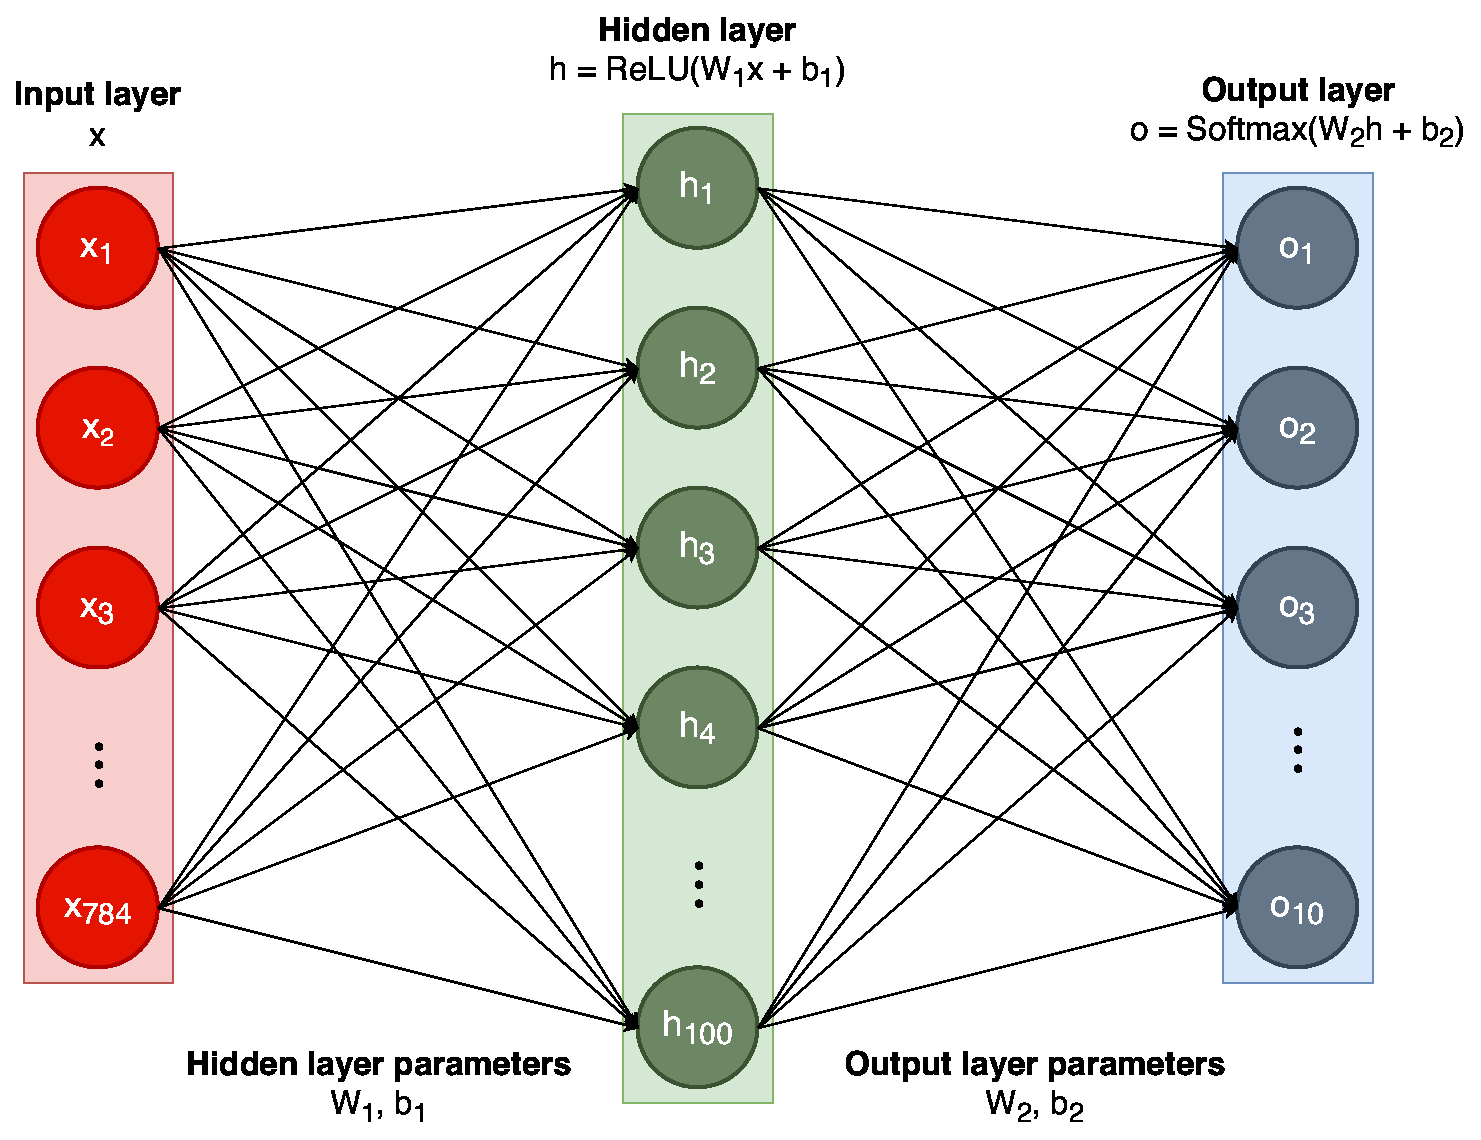
\includegraphics[width=1\textwidth]{Fig1.eps}
  \caption{The neural network with a hidden layer and an output layer}
\label{fig:back:model}
\end{figure}

This section describes two different forms of TensorFlow DL models written in
Python.
TensorFlow provides two major version libraries: TensorFlow 1.x published in
2016 and TensorFlow 2.x published in 2019. 
DL models significantly differ in their forms depending on which library
they use. 
On TensorFlow 1.x, model engineers manually construct models as computational
graphs using tensor variables and operations and execute them lazily  for
training and inference on an encapsulated environment
called {\it session}.
%The first version is TensorFlow 1.x published in 2016.
%TensorFlow 1.x provides APIs for defining tensor variables and operations
%between them.
%Developers manually define the model structure, the model operations 
%and training process using the TensorFlow 1.x APIs.
%On TensorFlow 1.x, developers need to manually define model structures, model
%operations, and their training process using APIs for defining tensor variables
%and operations between them.
%The second version is TensorFlow 2.x published in 2019.
On the other hand, TensorFlow 2.x supports the eager execution that executes
all tensor operations as they occur in code. 
With the eager execution feature, engineers no longer need to construct
computational graphs and use encapsulated environments.
%developers to use plain Python syntax to define the model
%operations and the training process.
In addition, TensorFlow 2.x integrates with the Keras library, a layer-based
deep learning model library that provides a convenient interface to construct
models.
%As a result, the models written in TensorFlow 1.x and TensorFlow 2.x are
%significantly differ in their forms. 

Figure~\ref{fig:back:model} illustrates an example neural network that
classifies input images into ten categories.
In the figure, vertical bars denote vectors of layers, circles denote data of
vectors, and direct edges denote data dependencies from source to destination
in vector operations.
%The model will get an input image of 784 pixels and classify it into one of ten
%output classes.
The network consists of three layers: an input, an output, and a hidden layer
between the two layers.
Each layer stores data into a vector, and the vector of a layer mutates into a
vector of another layer via vector operations.  
In the network, the input layer has a vector of length 784, and the data in the
vector is the pixels of an input image.
The hidden layer is parametrized by the two-dimensional weight matrix $W_1$ of
size 784 $\times$ 100 and the bias vector $b_1$ of length 100.
The hidden layer's vector is computed by multiplying the input layer
vector $x$ with the weight matrix $W_1$, adding the bias vector $b_1$, and
finally applying the ReLU activation function that makes the results non-zero
values.
The output layer is parametrized by the two-dimensional weight matrix $W_2$ of
size 100 $\times$ 10 and the bias vector $b_2$ of length 10.
The output layer's vector is computed by multiplying the hidden
layer vector $h$ with the weight matrix $W_2$, adding the bias vector $b_2$,
and finally applying the Softmax activation function that converts the ten data
to a probability distribution of the ten categories.
The weight matrices and the bias vectors in the network are model parameters,
and the training phase adjusts the model parameters repeatedly, to classify
input images correctly.
%The model structure is defined in terms of layers and operation between them.
%The layers are tensors of real values, which represent the signals and data.
%The model in the figure \ref{fig:back:model} has three layers;
%the input layer, the hidden layer, and the output layer.
%The layers are densely connected, which means that
%the layer outputs are computed by the linear transformation with 
%the weight matrices and the bias vectors, 
%and the non-linear activation functions. 
%The hidden layer is parametrized by the weight matrix
%$W_1$ of size (784, 100) and the bias vector $b_1$ of length 100.
%The hidden layer is computed by first multiplying the input layer vector $x$
%with the weight matrix $W_1$, adding the bias vector $b_1$, and finally applying
%the ReLU activation function to the result.
%The output layer is parametrized by the weight matrix $W_2$ of size (100, 10)
%and the bias vector $b_2$ of length 10.
%The output layer is computed by first multiplying the hidden layer vector $h$
%with the weight matrix $W_2$, adding the bias vector $b_2$, and finally applying
%the Softmax activation function to the result.
%The weight matrices and the bias vectors are called the model parameters 
%as their values are updated during the training process.
%The hidden layer is a vector of length 100.
%The output layer is a vector of length 10, and each vector element represents
%the probability of the input image classified into the corresponding class.

%We describe TensorFlow 1.x and 2.x versions with code examples that define
%the same model and the same training process.
%The code examples define the neural network model illustrated
%in the figure \ref{fig:back:model}.
%The model will get an input image of 784 pixels and classify it into one of ten
%output classes.
 
%The model structure is defined in terms of layers and operation between them.
%The layers are tensors of real values, which represent the signals and data.
%The model in the figure \ref{fig:back:model} has three layers;
%the input layer, the hidden layer, and the output layer.
%The input layer is a vector of length 784, which represents the input image
%of 784 pixels.
%The hidden layer is a vector of length 100.
%The output layer is a vector of length 10, and each vector element represents 
%the probability of the input image classified into the corresponding class.
%The layers are densely connected, which means that
%the layer outputs are computed by the linear transformation with 
%the weight matrices and the bias vectors, 
%and the non-linear activation functions. 
%The hidden layer is parametrized by the weight matrix
%$W_1$ of size (784, 100) and the bias vector $b_1$ of length 100.
%The hidden layer is computed by first multiplying the input layer vector $x$
%with the weight matrix $W_1$, adding the bias vector $b_1$, and finally applying
%the ReLU activation function to the result.
%The output layer is parametrized by the weight matrix $W_2$ of size (100, 10)
%and the bias vector $b_2$ of length 10.
%The output layer is computed by first multiplying the hidden layer vector $h$
%with the weight matrix $W_2$, adding the bias vector $b_2$, and finally applying
%the Softmax activation function to the result.
%The weight matrices and the bias vectors are called the model parameters 
%as their values are updated during the training process.

%The model is trained by the gradient descent algorithm. 
%The gradient descent algorithm is an iterative optimization algorithm
%that computes the gradients of model parameters to update their values toward
%local minimum of the loss function.
%The loss function defines the metric of the difference between the model 
%output and answer label.
%Thus, approaching the local minumum of the loss function means that the
%the gradient descent trains the model to return the output similar to the
%correct answer.
%In DL model training, the gradient descent is repeated against several
%training batches. Given a training input batch, the algorithm first computes
%the model loss with forward propagation then computes the gradients of the
%model parameters with backpropagation. The algorithm applies the gradients
%to update the model parameters, thus approaching to the minumum loss.

\begin{figure}[ht!]\centering
  \begin{lstlisting}[style=mpython]
import tensorflow.compat.v1 as tf

dataset = ...

x = tf.placeholder(tf.float32, [BATCH_SIZE, 784])
y = tf.placeholder(tf.float32, [BATCH_SIZE, 10]) 

W_1 = tf.Variable(tf.random_uniform([784, 100]))
b_1 = tf.Variable(tf.zeros([100]))
layer_1 = tf.nn.relu(tf.matmul(x, W_1) + b_1)

W_2 = tf.Variable(tf.random_uniform([100, 10]))
b_2 = tf.Variable(tf.zeros([10]))
layer_2 = tf.nn.softmax(tf.matmul(layer_1, W_2) + b_2)

loss = -tf.reduce_sum(y * tf.log(layer_2), 1) # Categorical cross entropy 
train_op = tf.train.AdamOptimizer(0.001).minimize(loss)

with tf.Session() as sess:
  sess.run(tf.global_variables_initializer())
  for images, labels in dataset.take(10000): 
    sess.run(train_op, {x: images, y: labels}) \end{lstlisting}
  \caption{TensorFlow 1.x model example}
\label{fig:back:tf1}
\end{figure}

Figure~\ref{fig:back:tf1} shows a TensorFlow 1.x model for the example neural
network with the gradient descent training algorithm.
First, lines 5 to 14 define the network structure and the operations
between the layers.
Lines 5 and 6 first create two placeholder variables, {\tt x} and {\tt y},
where {\tt x} is a vector storing the pixel data of an input image, and {\tt y}
is a vector storing the answer for the classification of the input image. 
Lines 8 to 10 define the hidden layer.
Line 8 creates a randomly initialized weight matrix {\tt W\_1}, and line 9
creates a zero-initialized bias vector {\tt b\_1}.
Then, the {\tt Variable} API wraps the matrix and the bias vector.
The {\tt Variable} API creates a model parameter of which internal values are
modifiable during training.
Line 10 defines the operation of the hidden layer. It first multiplies the
input vector {\tt x} with the weight matrix {\tt W\_1}, then adds the bias {\tt
b\_1}, and finally applies the ReLU activation function. 
Note that the line does not perform the operation but only defines how
the input data mutates into the hidden layer's data while executing the
model.
Lines 12 to 14 define the output layer.
Similar to lines 8 and 9, lines 12 and 13 define a randomly-initialized
weight matrix {\tt W\_2}, and a zero-initialized bias vector {\tt b\_2}, as
model parameters of the output layer.
Then, line 14 defines the operation that
multiplies the hidden layer output with
the weight {\tt W\_2}, adds the bias vector {\tt b\_2}, and finally applies the
{\tt softmax} activation function.


%As shown in the lines 5 to 14, developers must explicitly define
%the model components and oprations between them in TensorFlow 1.x model.

%Since the placeholder variables only specify the vector size of the input images
%and the labels; they will be replaced with actual values of the training
%data during the training process. 

%To define a neural network model in TensorFlow 1.x, 
%developers must explicitly define the model structure
%and the operations between the layers. 
%The developers also must manually start the training loop by explicitly
%accessing the TensorFlow runtime with dedicated APIs.

%The lines 8 to 10 defines the hidden layer.
%The line 8 uses the {\tt random\_uniform} API to create 
%a random weight matrix of size 784 by 100, 
%and the line 9 uses the {\tt zero} API to create a zero-vector of size 100.
%Then, the lines 8 and 9 wrap the weight matrix and the bias vector with
%{\tt Variable} API.
%The {\tt Variable} API creates a TensorFlow variable that can be later modified
%during the runtime. It is usually used to define a model 
%parameter, whose value is changed during the training process.
%Thus, the lines 8 and 9 create the weight and bias parameters for the
%hidden layer which have correct sizes and are modifiable during the 
%training process.
%The line 10 manually defines the operations of the hidden layer. 
%Note that the line does not actually compute the operations,
%but only define the operations that will be computed during the training.

After constructing the neural network, the code defines the training algorithm
in lines 16 and 17.
Line 16 defines the categorical cross-entropy loss function that
quantifies the degree of difference between the output data of {\tt layer\_2}
and the answer {\tt y}.
Line 17, then, creates an object of the {\tt AdamOptimizer} that is an
implementation of the Adam gradient descent algorithm~\cite{kingma2014adam}.
The {\tt minimize} method of the object generates a training operation that
updates model parameters using the Adam gradient descent algorithm to minimize
the loss calculated by the loss function.

%The lines 16 and 17 defines the loss function and the training operation. 
%The line 16 defines the loss function between the model output {\tt layer\_2} 
%and the answer label {\tt y} with categorial cross entropy function.
%The line 17 defines the training operation for the model.
%The line first calls the {\tt AdamOptimizer} constructor
%function to create an optimizer object.
%The optimizer objects in TensorFlow are abstractions of the gradient
%descent algorithms.
%For instance, the {\tt AdamOptimizer} abstracts a Adam gradient descent
%algorithm. % todo: cite Adam g.d.
%Then the {\tt minimize} method defines the training operation that updates the
%TensorFlow variables via the gradient descent on the first argument.
%Thus, the line 17 defines the operation of a single training step,
%which optimizes the model parameters via gradient descent to the loss gradient.

Lines 19 to 22 train the model in a session.
Line 19 creates a {\tt Session} object that provides an encapsulated
environment storing model parameters.
%that provides the {\tt run} method to execute the network's operations in an
%encapsulated environment.
%The line 20 calls the {\tt run} method with a global variable initializer
%to initialize model parameters of the network.
Line 20 calls the {\tt run} method of the object with a global variable
initializer to initialize all the model parameters of the model in the
encapsulated environment.
%The {\tt Session} object provides the {\tt run} method that can invoke
%computation of TensorFlow operations.
%Before the training computation starts,
%the TensorFlow variables in the model and the optimizer should be initialized.
%Note that the optimizer object implicitly introduces the variables which are 
%used for the internal computation.
%After the variables are initialized, the line 21 uses the {\tt for} loop
%to iterate over the dataset and get training input data. 
Lines 21 and 22 then train the model in a loop that executes the training
operation {\tt train\_op} with the input data {\tt x} and {\tt y} by iterating
over the ten thousand input datasets obtained from {\tt dataset.take(10000)}.

%The number of training data is specified by the {\tt take} API of the
%dataset object.
%Finally, the line 22 calls the {\tt run} method to
%invoke computation of the training operation {\tt train\_op}.
